\section{Model predictions errors for counties in the United States}

When applied to data for different counties in the \gls{US}, all three versions of the model also showed consistent results and predicted similar trends across all locations.
Similar to the results obtained from the experiments with country-level data, all versions were able to simultaneously predict the number of cases in different categories with high accuracy for up to 14 days.
After the 14-day mark, the predictions errors started to increase as more uncertainties were accumulated when the dynamics were extrapolated further into the future.
Additionally, the results once again indicated that our method of encoding data from Facebook into the model did not improve the long-term predicting performance of the model.

When predicting the number of deaths of the disease, \autoref{tab:errors-us-counties-deaths} shows that the baseline model significantly outperformed the other two versions with data for Cook (Illinois) and Los Angeles (California) on all forecast horizons.
Here, the predictions errors of the baseline model were less than half of the predictions errors from the other two versions across all metrics.
On the other hand, the third version of the model achieved the lowest error when predicting for Harris (Texas) on all horizons.
While the third version had the best performance across all metrics when predicting for Maricopa (Arizona) on 7-day and 14-day horizons, at the 21-day horizon, its performance started to diminish.
With a 21-day horizon, the baseline model's predictions for Maricopa (Arizona) had the lowest \gls{RMSE} and with the other metrics closely followed that of the third version.
Then with a 28-day horizon, the baseline model completely outperformed the third version across all metrics.

On the predictions for the number of new cases, \autoref{tab:errors-us-counties-new-cases} shows results similar to the performance of the different versions when predicting the number of deaths.
Here, the baseline model significantly outperformed the others across all metrics when predicting the number of new cases for Cook (Illinois) and Los Angeles (California) for all forecast horizons.
When predicting the number of new cases for Harris (Texas), the third version had the best performance on the 7-day horizon, however, with 14-day and 21-day horizons, the third version only had the lowest errors with the \gls{MAE} and \gls{RMSE} metrics, whereas the best \glspl{MAPE} for those horizons were achieved by the baseline model.
The baseline model additionally had the lowest \gls{MAE} and \gls{MAPE} when predicting for Harris (Texas) on the 28-day horizon, while the lowest \gls{RMSE} was produced by the third version.
Furthermore, the third version of the model had the lowest errors across all metrics when predicting for Maricopa (Arizona) for the 7-day and 21-day horizons.
With the 14-day predictions for Maricopa (Arizona), the second version of the model had the lowest predictions error with \gls{RMSE} while the third version of the model had the lowest predictions error with \gls{MAE} and \gls{MAPE}.
Lastly, with the 28-days predictions for Maricopa (Arizona), the second version had the lowest errors across all metrics.

When predicting the number of cumulative cases, \autoref{tab:errors-us-counties-total-cases} shows that for the 7-day forecast horizon, the baseline model performed best with data for Los Angeles (California), while the third version had the lowest predictions errors for all the other locations.
For the 14-day and 21-day forecast horizons, the third version had the lowest predictions errors for Harris (Texas) and Maricopa (Arizona), while the baseline had the lowest predictions errors for Cook (Illinois) and Los Angeles (California).
Finally, for the 28-day forecast horizon, the baseline only achieved the best performance on data for Harris (Texas) and the third version performed best for all the other locations.

Overall, the results show that there was not a significant difference in the long-term forecasting performance across the three different versions.
In addition, it was observed from the errors tables that the model's performance was largely dependent on the chosen location where the baseline model performed generally better with data for Cook (Illinois) and Los Angeles (California), and the third version performed generally better with data for Harris (Texas) and Maricopa (Arizona).

% ERRORS

\begin{landscape}
\begin{table}[!htb]
    \centering
    \begin{tabular}{| c | c | c | c | c | c | c | c | c | c | c |}
        \multirow{2}{*}{Days}
            & \multirow{2}{*}{Loc.}
            & \multicolumn{3}{c |}{Baseline}
            & \multicolumn{3}{c |}{2nd. Version}
            & \multicolumn{3}{c |}{3rd. Version} \\ \cline{3-11}
            & & MAE & MAPE & RMSE & MAE & MAPE & RMSE & MAE & MAPE & RMSE \\ \hline\hline

        \multirow{4}{*}{7}
            & Cook, IL & \textbf{5.847} & \textbf{0.055} & \textbf{6.291} & 18.390 & 0.173 & 19.257 & 21.309 & 0.200 & 22.031 \\
            & Harris, TX & 46.021 & 0.666 & 50.000 & 38.705 & 0.560 & 43.120 & \textbf{32.571} & \textbf{0.471} & \textbf{36.267} \\
            & Los Angeless, CA & \textbf{28.781} & \textbf{0.115} & \textbf{31.633} & 51.605 & 0.206 & 54.813 & 50.488 & 0.202 & 53.633 \\
            & Maricopa, AZ & 39.739 & 0.374 & 40.227 & 38.180 & 0.360 & 38.746 & \textbf{36.632} & \textbf{0.345} & \textbf{37.215} \\ \hline

        \multirow{4}{*}{14}
            & Cook, IL & \textbf{13.181} & \textbf{0.123} & \textbf{15.800} & 31.772 & 0.297 & 35.375 & 34.551 & 0.323 & 37.832 \\
            & Harris, TX & 95.339 & 1.355 & 111.180 & 87.944 & 1.249 & 104.920 & \textbf{74.100} & \textbf{1.052} & \textbf{88.397} \\
            & Los Angeless, CA & \textbf{54.539} & \textbf{0.217} & \textbf{61.814} & 87.975 & 0.350 & 97.176 & 86.045 & 0.343 & 95.029 \\
            & Maricopa, AZ & 55.439 & 0.519 & 58.393 & 54.897 & 0.514 & 58.269 & \textbf{53.215} & \textbf{0.498} & \textbf{56.632} \\ \hline

        \multirow{4}{*}{21}
            & Cook, IL & \textbf{21.380} & \textbf{0.199} & \textbf{25.491} & 45.720 & 0.426 & 51.581 & 48.620 & 0.453 & 54.215 \\
            & Harris, TX & 158.343 & 2.205 & 189.162 & 152.570 & 2.123 & 185.661 & \textbf{127.313} & \textbf{1.772} & \textbf{154.368} \\
            & Los Angeless, CA & \textbf{82.513} & \textbf{0.327} & \textbf{95.410} & 126.976 & 0.503 & 143.413 & 123.921 & 0.491 & 139.857 \\
            & Maricopa, AZ & 76.472 & 0.711 & \textbf{83.882} & 77.590 & 0.721 & 86.019 & \textbf{75.672} & \textbf{0.703} & 84.128 \\ \hline

        \multirow{4}{*}{28}
            & Cook, IL & \textbf{29.629} & \textbf{0.275} & \textbf{35.088} & 59.121 & 0.549 & 66.872 & 62.355 & 0.579 & 69.979 \\
            & Harris, TX & 227.124 & 3.099 & 272.682 & 225.190 & 3.070 & 274.928 & \textbf{184.261} & \textbf{2.513} & \textbf{223.061} \\
            & Los Angeless, CA & \textbf{117.110} & \textbf{0.461} & \textbf{138.626} & 171.721 & 0.677 & 197.699 & 167.210 & 0.659 & 192.284 \\
            & Maricopa, AZ & \textbf{101.192} & \textbf{0.933} & \textbf{114.101} & 104.663 & 0.965 & 119.408 & 102.385 & 0.944 & 117.066 \\ \hline
    \end{tabular}
    \caption{Out-of-sample errors of the model's predictions on the number of deaths for the counties in the United States. The lowest errors for each evaluation metrics at each location are highlighted.}
    \label{tab:errors-us-counties-deaths}
\end{table}
\end{landscape}

\begin{landscape}
\begin{table}[!htb]
    \centering
    \begin{tabular}{| c | c | c | c | c | c | c | c | c | c | c |}
        \multirow{2}{*}{Days}
            & \multirow{2}{*}{Loc.}
            & \multicolumn{3}{c |}{Baseline}
            & \multicolumn{3}{c |}{2nd. Version}
            & \multicolumn{3}{c |}{3rd. Version} \\ \cline{3-11}
            & & MAE & MAPE & RMSE & MAE & MAPE & RMSE & MAE & MAPE & RMSE \\ \hline\hline

        \multirow{4}{*}{7}
            & Cook, IL & \textbf{22.545} & \textbf{2.377} & \textbf{28.432} & 55.668 & 6.041 & 66.778 & 41.352 & 4.467 & 55.134 \\
            & Harris, TX & 1022.438 & 30.850 & 1193.354 & 1093.142 & 32.772 & 1280.746 & \textbf{797.754} & \textbf{26.782} & \textbf{865.731} \\
            & Los Angeless, CA & \textbf{981.461} & \textbf{20.945} & \textbf{1140.886} & 1126.805 & 24.141 & 1297.286 & 1082.929 & 23.181 & 1248.996 \\
            & Maricopa, AZ & 95.129 & 4.730 & 99.906 & 19.956 & 0.987 & 23.867 & \textbf{19.382} & \textbf{0.968} & \textbf{21.617} \\ \hline

        \multirow{4}{*}{14}
            & Cook, IL & \textbf{35.341} & \textbf{3.517} & \textbf{45.173} & 90.017 & 9.156 & 101.192 & 59.667 & 6.104 & 68.594 \\
            & Harris, TX & 890.257 & \textbf{28.652} & 1093.096 & 984.436 & 30.810 & 1205.333 & \textbf{790.239} & 30.445 & \textbf{874.964} \\
            & Los Angeless, CA & \textbf{698.901} & \textbf{15.302} & \textbf{950.789} & 802.626 & 17.610 & 1085.485 & 768.943 & 16.918 & 1038.125 \\
            & Maricopa, AZ & 136.129 & 6.883 & 172.143 & 69.022 & 3.427 & \textbf{94.846} & \textbf{62.939} & \textbf{3.176} & 95.737 \\ \hline

        \multirow{4}{*}{21}
            & Cook, IL & \textbf{70.168} & \textbf{7.131} & \textbf{92.661} & 136.784 & 14.489 & 177.086 & 96.828 & 10.550 & 144.579 \\
            & Harris, TX & 715.160 & \textbf{23.718} & 932.114 & 963.073 & 32.888 & 1132.567 & \textbf{671.354} & 26.827 & \textbf{775.119} \\
            & Los Angeless, CA & \textbf{477.179} & \textbf{10.682} & \textbf{776.682} & 557.786 & 12.785 & 887.881 & 584.712 & 14.463 & 857.916 \\
            & Maricopa, AZ & 139.674 & 6.888 & 169.314 & 92.801 & 4.357 & 129.381 & \textbf{76.112} & \textbf{3.609} & \textbf{116.774} \\ \hline

        \multirow{4}{*}{28}
            & Cook, IL & \textbf{83.696} & \textbf{8.105} & \textbf{119.396} & 184.792 & 19.135 & 230.863 & 139.144 & 14.665 & 190.726 \\
            & Harris, TX & \textbf{605.536} & \textbf{20.796} & 824.160 & 982.211 & 35.537 & 1123.076 & 689.374 & 28.746 & \textbf{779.813} \\
            & Los Angeless, CA & \textbf{412.908} & \textbf{11.617} & \textbf{686.484} & 498.917 & 14.897 & 794.109 & 546.785 & 17.824 & 784.312 \\
            & Maricopa, AZ & 217.947 & 11.510 & 271.885 & \textbf{104.125} & \textbf{5.223} & \textbf{134.620} & 109.935 & 5.689 & 149.951 \\ \hline
    \end{tabular}
    \caption{Out-of-sample errors of the model's predictions on the number of new cases for the counties in the United States. The lowest errors for each evaluation metrics at each location are highlighted.}
    \label{tab:errors-us-counties-new-cases}
\end{table}
\end{landscape}

\begin{landscape}
\begin{table}[!htb]
    \centering
    \begin{tabular}{| c | c | c | c | c | c | c | c | c | c | c |}
        \multirow{2}{*}{Days}
            & \multirow{2}{*}{Loc.}
            & \multicolumn{3}{c |}{Baseline}
            & \multicolumn{3}{c |}{2nd. Version}
            & \multicolumn{3}{c |}{3rd. Version} \\ \cline{3-11}
            & & MAE & MAPE & RMSE & MAE & MAPE & RMSE & MAE & MAPE & RMSE \\ \hline\hline

        \multirow{4}{*}{7}
            & Cook, IL & 678.757 & 0.117 & 679.641 & 750.786 & 0.130 & 761.605 & \textbf{595.890} & \textbf{0.103} & \textbf{604.919} \\
            & Harris, TX & 2429.798 & 0.520 & 3193.800 & 2629.532 & 0.562 & 3482.363 & \textbf{1535.176} & \textbf{0.333} & \textbf{1736.348} \\
            & Los Angeless, CA & \textbf{2351.443} & \textbf{0.172} & \textbf{2920.659} & 2898.771 & 0.212 & 3633.093 & 2545.519 & 0.186 & 3107.429 \\
            & Maricopa, AZ & 1491.513 & 0.242 & 1510.229 & 974.924 & 0.159 & 975.073 & \textbf{410.099} & \textbf{0.067} & \textbf{412.091} \\ \hline

        \multirow{4}{*}{14}
            & Cook, IL & \textbf{612.953} & \textbf{0.105} & \textbf{621.265} & 1129.956 & 0.194 & 1212.272 & 874.273 & 0.150 & 928.652 \\
            & Harris, TX & 5883.932 & 1.224 & 6993.098 & 6824.524 & 1.419 & 8209.270 & \textbf{2209.289} & \textbf{0.465} & \textbf{2506.827} \\
            & Los Angeless, CA & \textbf{5141.081} & \textbf{0.371} & \textbf{5985.620} & 6376.008 & 0.460 & 7440.514 & 5501.848 & 0.397 & 6381.884 \\
            & Maricopa, AZ & 2026.365 & 0.325 & 2112.334 & 963.663 & 0.155 & 969.336 & \textbf{480.406} & \textbf{0.077} & \textbf{492.111} \\ \hline

        \multirow{4}{*}{21}
            & Cook, IL & \textbf{465.474} & \textbf{0.080} & \textbf{519.420} & 1659.534 & 0.282 & 1879.133 & 1219.233 & 0.207 & 1359.485 \\
            & Harris, TX & 7611.514 & 1.553 & 8583.826 & 9913.906 & 2.017 & 11519.766 & \textbf{1664.322} & \textbf{0.348} & \textbf{2097.628} \\
            & Los Angeless, CA & \textbf{6242.229} & \textbf{0.447} & \textbf{6903.758} & 7690.419 & 0.551 & 8509.198 & 6313.624 & 0.452 & 6943.113 \\
            & Maricopa, AZ & 2549.187 & 0.402 & 2705.335 & 767.923 & 0.123 & 826.909 & \textbf{396.265} & \textbf{0.063} & \textbf{425.505} \\ \hline

        \multirow{4}{*}{28}
            & Cook, IL & \textbf{486.965} & \textbf{0.083} & \textbf{548.673} & 2493.195 & 0.420 & 3000.083 & 1869.379 & 0.315 & 2260.015 \\
            & Harris, TX & 8785.001 & 1.760 & 9652.091 & 13119.518 & 2.612 & 15167.205 & \textbf{2479.698} & \textbf{0.499} & \textbf{3145.165} \\
            & Los Angeless, CA & 6715.207 & 0.478 & 7232.734 & 7974.478 & 0.568 & 8596.755 & \textbf{6094.396} & \textbf{0.435} & \textbf{6615.172} \\
            & Maricopa, AZ & 3327.537 & 0.517 & 3705.984 & 670.792 & 0.107 & 754.504 & \textbf{452.858} & \textbf{0.071} & \textbf{533.121} \\ \hline
    \end{tabular}
    \caption{Out-of-sample errors of the model's predictions on the number of cumulative cases for the counties in the United States. The lowest errors for each evaluation metrics at each location are highlighted.}
    \label{tab:errors-us-counties-total-cases}
\end{table}
\end{landscape}

\subsection{Reproduction number and fatality rate}

Considering \autoref{fig:R0-and-fatality-cook}, all three versions were able to learn the same trend for the effective reproduction number where it decreased sharply to below $1$ for the first 15 time steps and then sharply increased for a short period of 10 time steps before gradually decreased until the end of the simulation.
At the first few time steps, both the baseline model and the third version predicted a very low value for the effective reproduction number before rapidly increasing to a maximum value.
The reason for this behavior was because in the dataset for Cook (Illinois) the number of new cases at the beginning of the chosen period was on the decrease for a few days before it increased again.
Looking at \autoref{fig:fit-us-counties}, it can be seen that both the baseline model and the third version closely follow the declining number of new cases for the first few days, resulting in the low effective reproduction number in the beginning.
On the other hand, the second version did not have a good fit for this period, hence the effective reproduction number given by the second version was different from the other two versions.
Moreover, the max effective reproduction number predicted by the second version was higher at around $2.5$ whereas the other versions had the max effective reproduction number at around $2$.
With regards to the fatality rate, both the baseline model and the third version learned a similar trend where the fatality rate started at around $0.045$ and exponentially decreased as time went on.
Because of the high effective reproduction number that was predicted at the beginning of the simulation, the fatality rate predicted by the second version was lower for the first $20$ time steps compared to the baseline model and the third version.
For the period after the first $20$ time steps, the fatality rate predicted by the second version followed a decreasing trend similar to the fatality rate predicted by the other two models.

\begin{figure}[!htb]
    \centering

    \begin{subfigure}[b]{\linewidth}
        \centering
        \begin{subfigure}[b]{0.4\linewidth}
            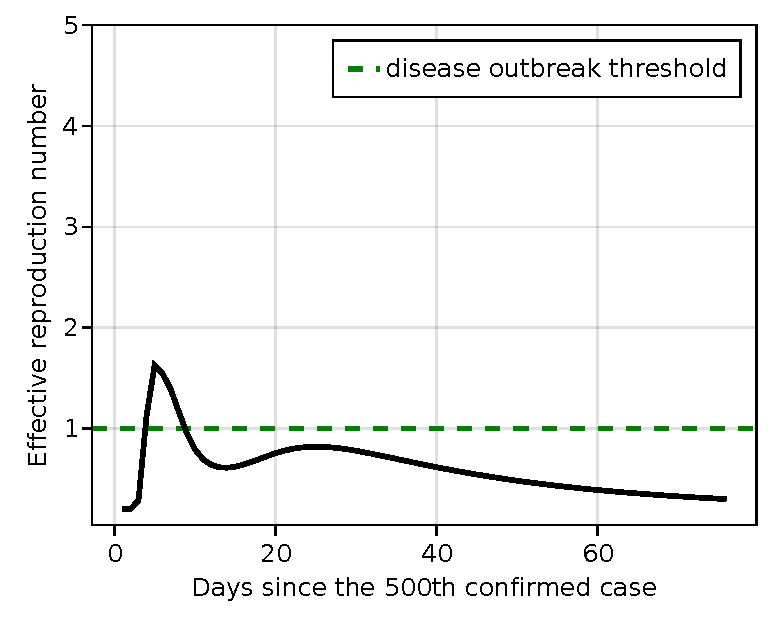
\includegraphics[width=\linewidth]{baseline/cook_il/20211215163025.baseline.cook_il.R_effective.pdf}
        \end{subfigure}
        \begin{subfigure}[b]{0.4\linewidth}
            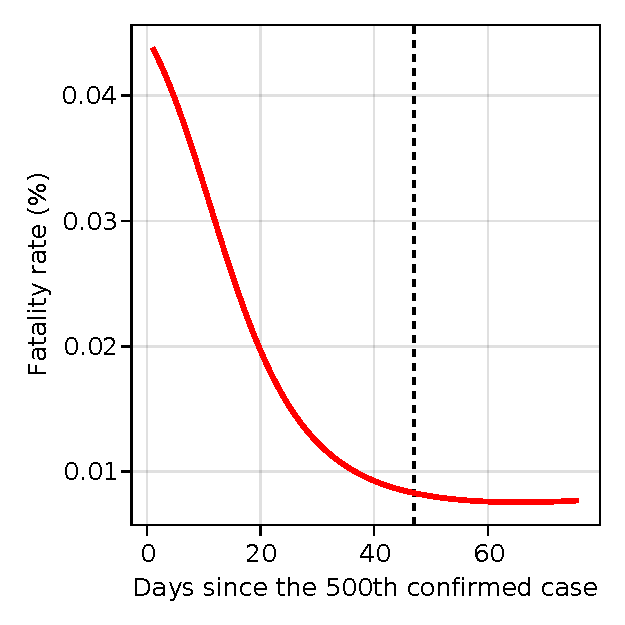
\includegraphics[width=\linewidth]{baseline/cook_il/20211215163025.baseline.cook_il.fatality_rate.pdf}
        \end{subfigure}
        \subcaption{Baseline model}
    \end{subfigure}

    \begin{subfigure}[b]{\linewidth}
        \centering
        \begin{subfigure}[b]{0.4\linewidth}
            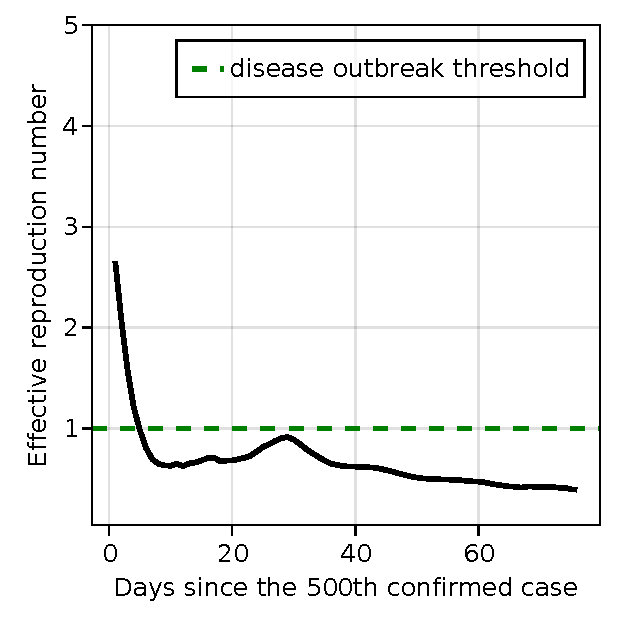
\includegraphics[width=\linewidth]{fb1/cook_il/20211216131821.fbmobility1.cook_il.R_effective.pdf}
        \end{subfigure}
        \begin{subfigure}[b]{0.4\linewidth}
            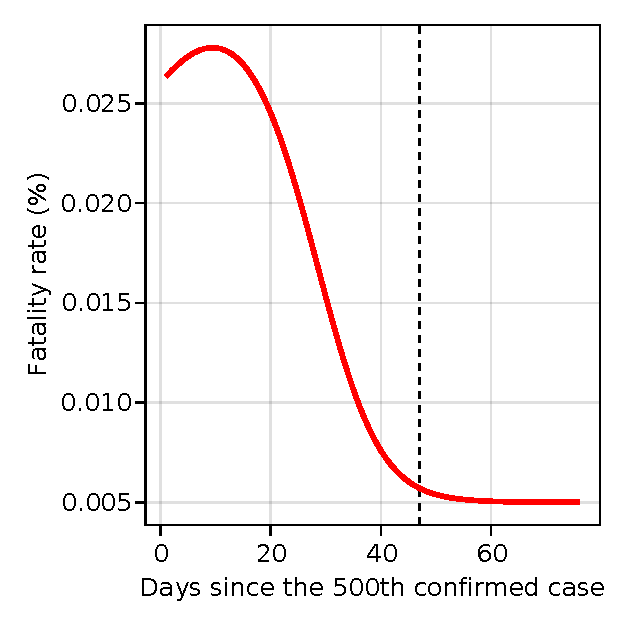
\includegraphics[width=\linewidth]{fb1/cook_il/20211216131821.fbmobility1.cook_il.fatality_rate.pdf}
        \end{subfigure}
        \subcaption{2nd. version}
    \end{subfigure}

    \begin{subfigure}[b]{\linewidth}
        \centering
        \begin{subfigure}[b]{0.4\linewidth}
            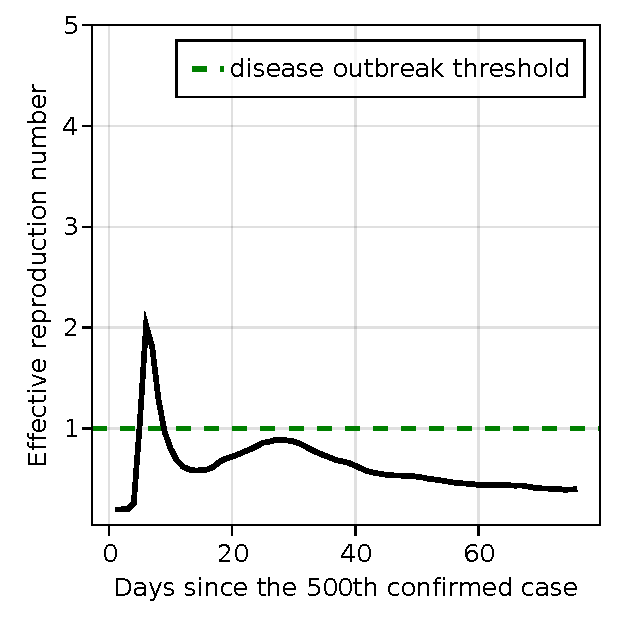
\includegraphics[width=\linewidth]{fb2/cook_il/20211216142727.fbmobility2.cook_il.R_effective.pdf}
        \end{subfigure}
        \begin{subfigure}[b]{0.4\linewidth}
            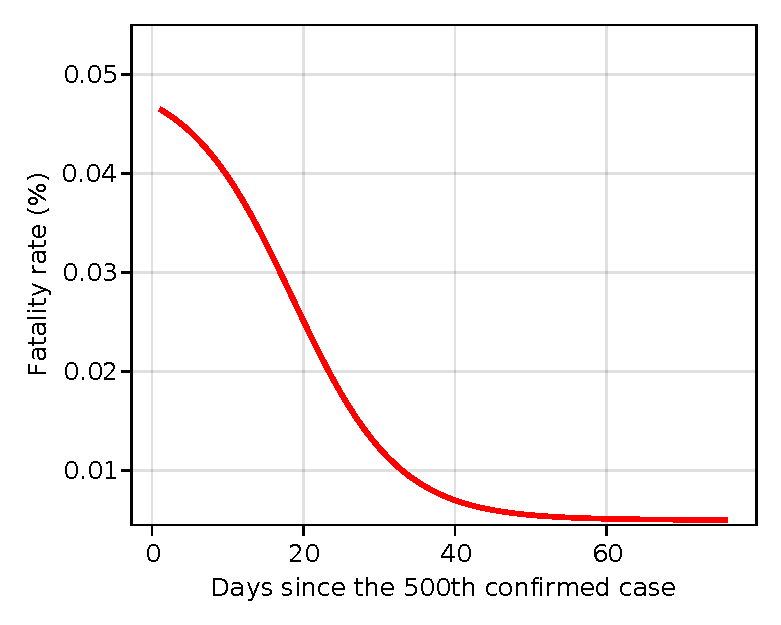
\includegraphics[width=\linewidth]{fb2/cook_il/20211216142727.fbmobility2.cook_il.fatality_rate.pdf}
        \end{subfigure}
        \subcaption{3rd. version}
    \end{subfigure}

    \caption{The effective reproduction number and the fatality rate for Cook (Illinois), learned by different versions of the model}
    \label{fig:R0-and-fatality-cook}
\end{figure}

For the county Harris (Texas), according to \autoref{fig:R0-and-fatality-harris}, all three versions predicted a similar trend in both the effective reproduction number and the fatality rate.
For the first few time steps, all three versions predicted a low effective reproduction number because of similar reasons to the case with the dataset for Cook (Illinois), which were illustrated in \autoref{fig:fit-us-counties}.
Both the baseline model and the third version predicted the maximum reproduction number of around $2.5$ while the second version predicted a much higher value of $4.5$.
After reaching the maximum effective reproduction number, all versions predicted a dropped in value to below $1$ at around the 15th time step followed by a sharp increase to above $1$ at the 25th time step before the effective reproduction number gradually decreased for the rest of the simulated period.
This trend of the effective reproduction number was similarly observed when trained with data for Cook (Illinois).
When predicting the fatality rate, all three versions showed similar results with the initial fatality rate at the 0th time step being the highest at around $0.045$, and the fatality rate dropped exponentially after the initial time step.

\begin{figure}[!htb]
    \centering

    \begin{subfigure}[b]{\linewidth}
        \centering
        \begin{subfigure}[b]{0.4\linewidth}
            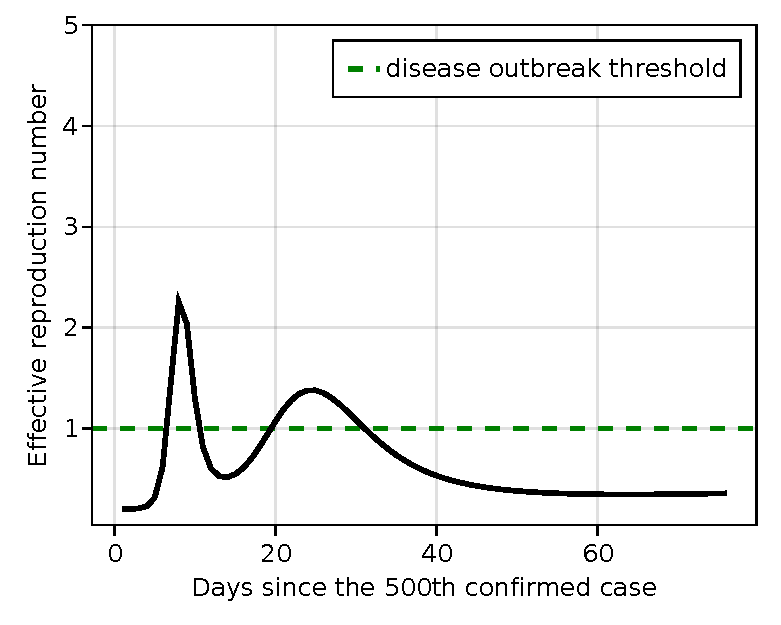
\includegraphics[width=\linewidth]{baseline/harris_tx/20211216154445.baseline.harris_tx.R_effective.pdf}
        \end{subfigure}
        \begin{subfigure}[b]{0.4\linewidth}
            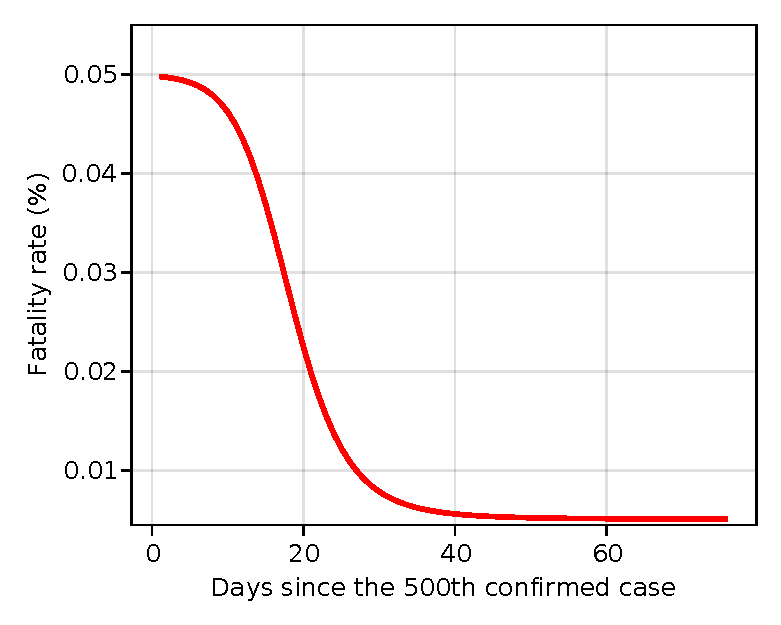
\includegraphics[width=\linewidth]{baseline/harris_tx/20211216154445.baseline.harris_tx.fatality_rate.pdf}
        \end{subfigure}
        \subcaption{Baseline model}
    \end{subfigure}

    \begin{subfigure}[b]{\linewidth}
        \centering
        \begin{subfigure}[b]{0.4\linewidth}
            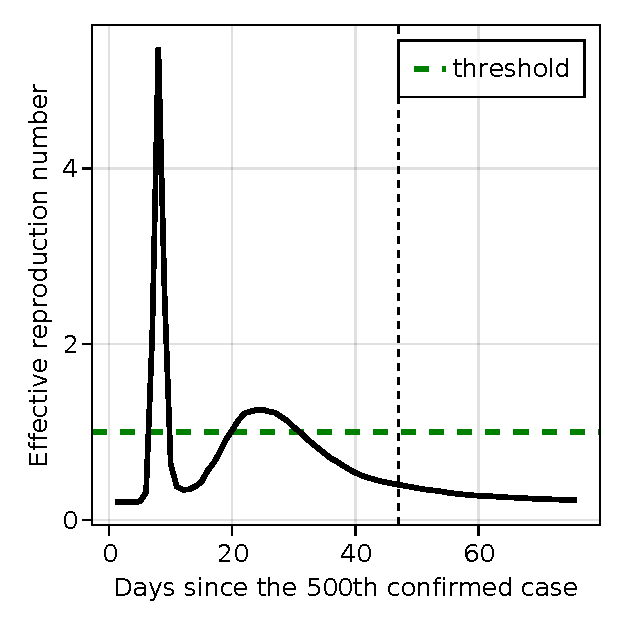
\includegraphics[width=\linewidth]{fb1/harris_tx/20211216231719.fbmobility1.harris_tx.R_effective.pdf}
        \end{subfigure}
        \begin{subfigure}[b]{0.4\linewidth}
            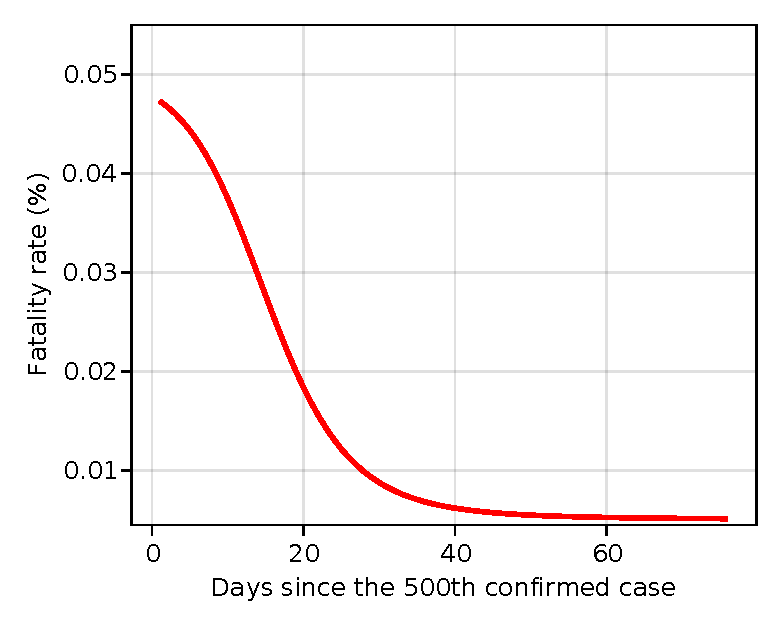
\includegraphics[width=\linewidth]{fb1/harris_tx/20211216231719.fbmobility1.harris_tx.fatality_rate.pdf}
        \end{subfigure}
        \subcaption{2nd. version}
    \end{subfigure}

    \begin{subfigure}[b]{\linewidth}
        \centering
        \begin{subfigure}[b]{0.4\linewidth}
            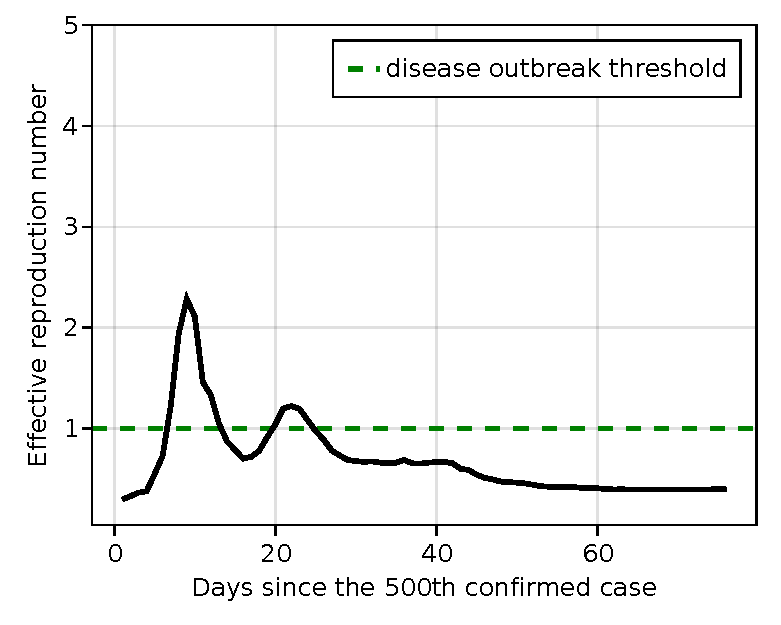
\includegraphics[width=\linewidth]{fb2/harris_tx/20211217204936.fbmobility2.harris_tx.R_effective.pdf}
        \end{subfigure}
        \begin{subfigure}[b]{0.4\linewidth}
            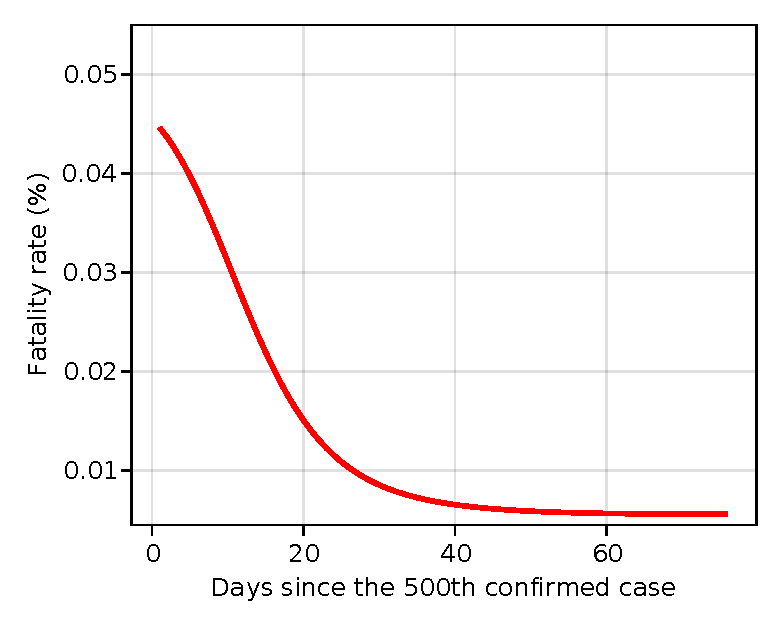
\includegraphics[width=\linewidth]{fb2/harris_tx/20211217204936.fbmobility2.harris_tx.fatality_rate.pdf}
        \end{subfigure}
        \subcaption{3rd. version}
    \end{subfigure}

    \caption{The effective reproduction number and the fatality rate for Harris (Texas) learned by different versions of the model}
    \label{fig:R0-and-fatality-harris}
\end{figure}

As illustrated in \autoref{fig:R0-and-fatality-losangeles}, after being trained with data for Los Angeles (California), the baseline model predicted the max effective reproduction number to be around $1.5$ whereas both the second version and the third version predicted a max value of around $1.25$.
Because of the initial decrease in the number of cases in the data for Los Angeles (California), the baseline model predicted a very low effective reproduction number for the first few time steps before predicting a sharp rise.
This behavior was also observed with the second version, although the initial predicted values were not as low as in the case with the baseline model.
However, in the third version, this low initial effective reproduction number was not predicted, and as a result, the third version's predictions for the number of new cases for Los Angeles (California) in the first few time steps did not decrease as sharply, as shown in \autoref{fig:fit-us-counties}.
After the initial max predicted value, all three versions showed a similar trend for the effective reproduction number that gradually decreased until the end of the simulation and passed the $1$ boundary at around the 20th time step.
Due to the low initial predicted effective reproduction number, the max fatality rate of $0.04$ predicted by the baseline model was much higher than the value predicted by the other two versions, which was around $0.025$.
Here, the predicted fatality rate in all three versions also followed an exponentially decreasing trend.

\begin{figure}[!htb]
    \centering

    \begin{subfigure}[b]{\linewidth}
        \centering
        \begin{subfigure}[b]{0.4\linewidth}
            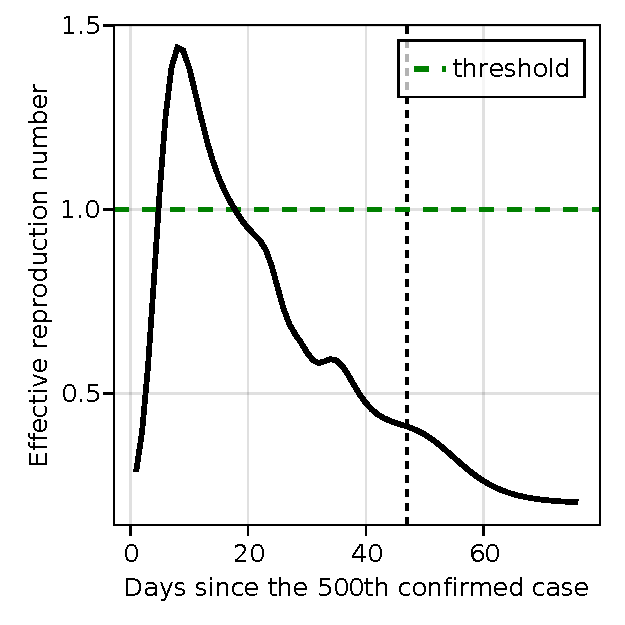
\includegraphics[width=\linewidth]{baseline/losangeles_ca/20211216124108.baseline.losangeles_ca.R_effective.pdf}
        \end{subfigure}
        \begin{subfigure}[b]{0.4\linewidth}
            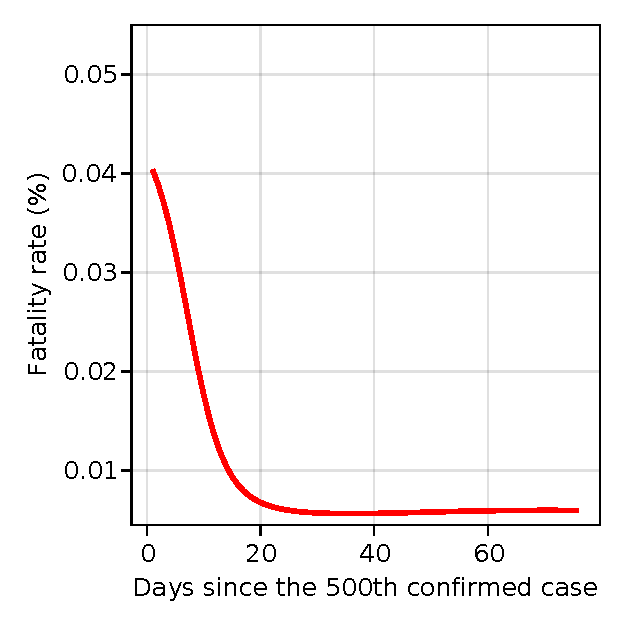
\includegraphics[width=\linewidth]{baseline/losangeles_ca/20211216124108.baseline.losangeles_ca.fatality_rate.pdf}
        \end{subfigure}
        \subcaption{Baseline model}
    \end{subfigure}

    \begin{subfigure}[b]{\linewidth}
        \centering
        \begin{subfigure}[b]{0.4\linewidth}
            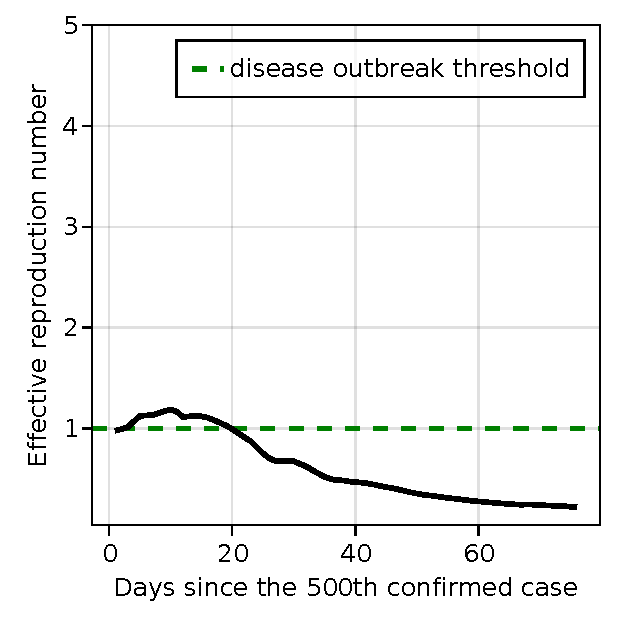
\includegraphics[width=\linewidth]{fb1/losangeles_ca/20211216180602.fbmobility1.losangeles_ca.R_effective.pdf}
        \end{subfigure}
        \begin{subfigure}[b]{0.4\linewidth}
            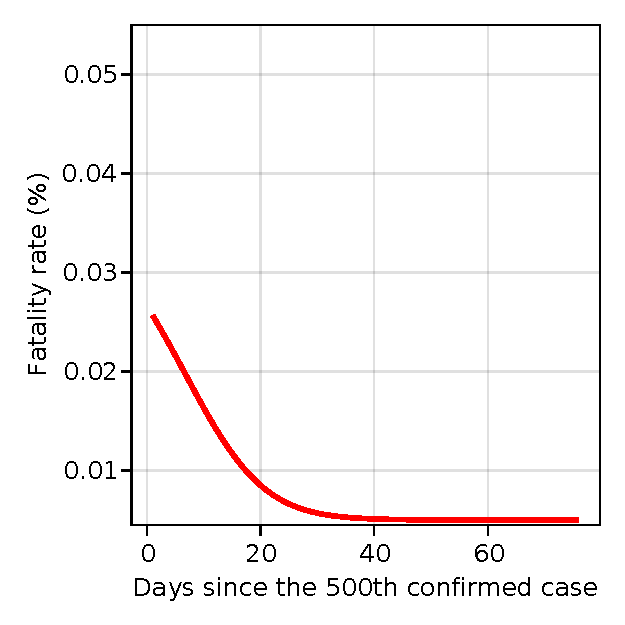
\includegraphics[width=\linewidth]{fb1/losangeles_ca/20211216180602.fbmobility1.losangeles_ca.fatality_rate.pdf}
        \end{subfigure}
        \subcaption{2nd. version}
    \end{subfigure}

    \begin{subfigure}[b]{\linewidth}
        \centering
        \begin{subfigure}[b]{0.4\linewidth}
            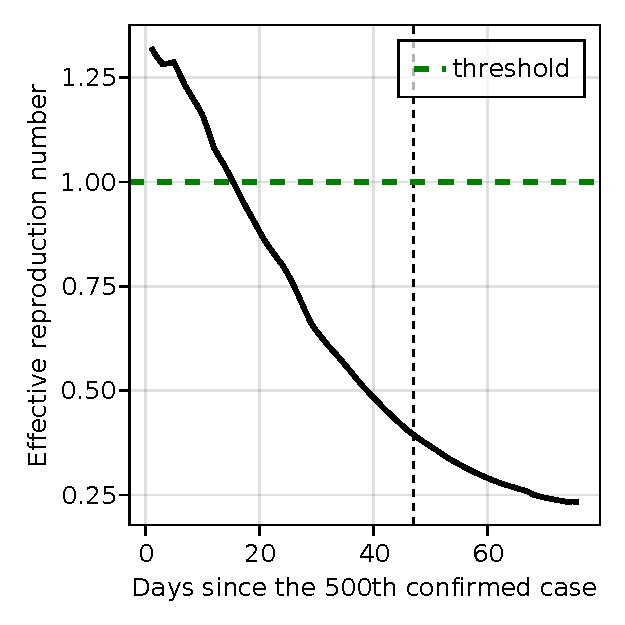
\includegraphics[width=\linewidth]{fb2/losangeles_ca/20211216142727.fbmobility2.losangeles_ca.R_effective.pdf}
        \end{subfigure}
        \begin{subfigure}[b]{0.4\linewidth}
            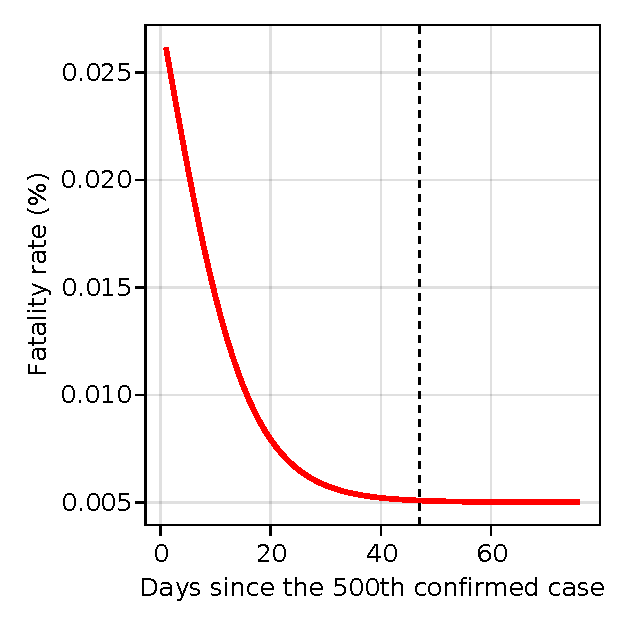
\includegraphics[width=\linewidth]{fb2/losangeles_ca/20211216142727.fbmobility2.losangeles_ca.fatality_rate.pdf}
        \end{subfigure}
        \subcaption{3rd. version}
    \end{subfigure}

    \caption{The effective reproduction number and the fatality rate for Los Angeles (California) learned by different versions of the model}
    \label{fig:R0-and-fatality-losangeles}
\end{figure}

For Maricopa (Arizona), all the versions predicted similar trends and values for both the effective reproduction number and the fatality rate.
The predicted effective production number was at its maximum at the 0th time step with a value of around $1.25$ which gradually drop off as time went on.
According to \autoref{fig:R0-and-fatality-maricopa}, the predicted effective reproduction number of all three versions crossed below $1$ at around the 10th time steps.
For the fatality rate, the maximum value of $0.05$ was predicted for the first few time steps before it exponentially decreased and stabilized until the end of the simulation.

\begin{figure}[!htb]
    \centering

    \begin{subfigure}[b]{\linewidth}
        \centering
        \begin{subfigure}[b]{0.4\linewidth}
            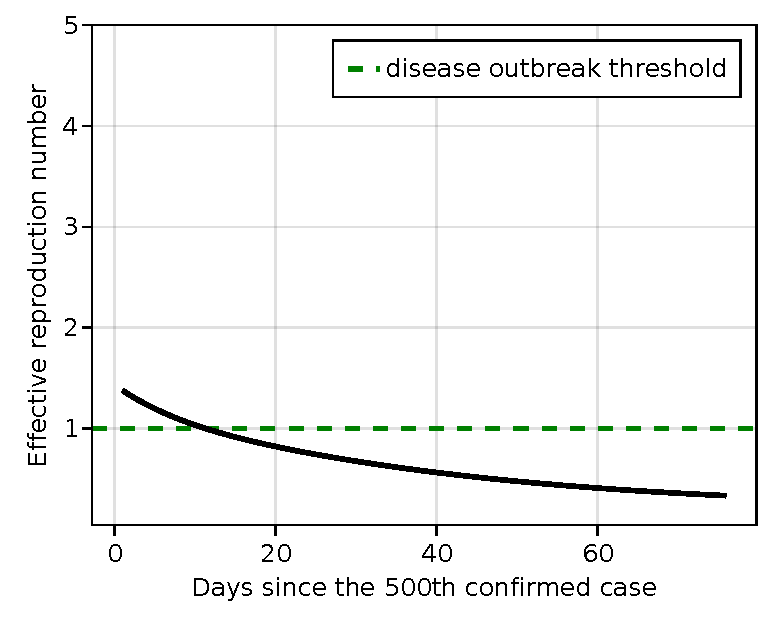
\includegraphics[width=\linewidth]{baseline/maricopa_az/20211216154445.baseline.maricopa_az.R_effective.pdf}
        \end{subfigure}
        \begin{subfigure}[b]{0.4\linewidth}
            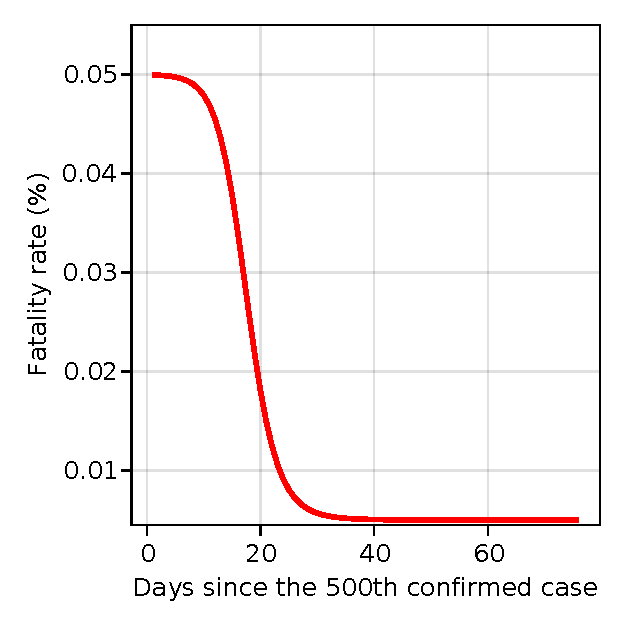
\includegraphics[width=\linewidth]{baseline/maricopa_az/20211216154445.baseline.maricopa_az.fatality_rate.pdf}
        \end{subfigure}
        \subcaption{Baseline model}
    \end{subfigure}

    \begin{subfigure}[b]{\linewidth}
        \centering
        \begin{subfigure}[b]{0.4\linewidth}
            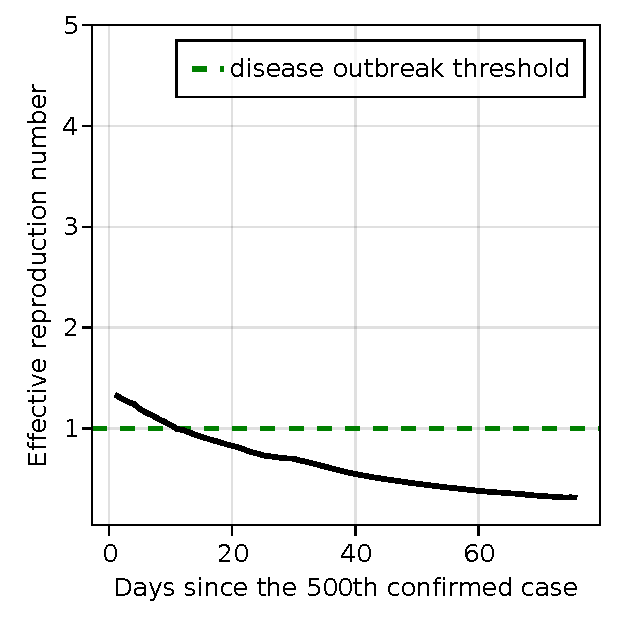
\includegraphics[width=\linewidth]{fb1/maricopa_az/20211216131821.fbmobility1.maricopa_az.R_effective.pdf}
        \end{subfigure}
        \begin{subfigure}[b]{0.4\linewidth}
            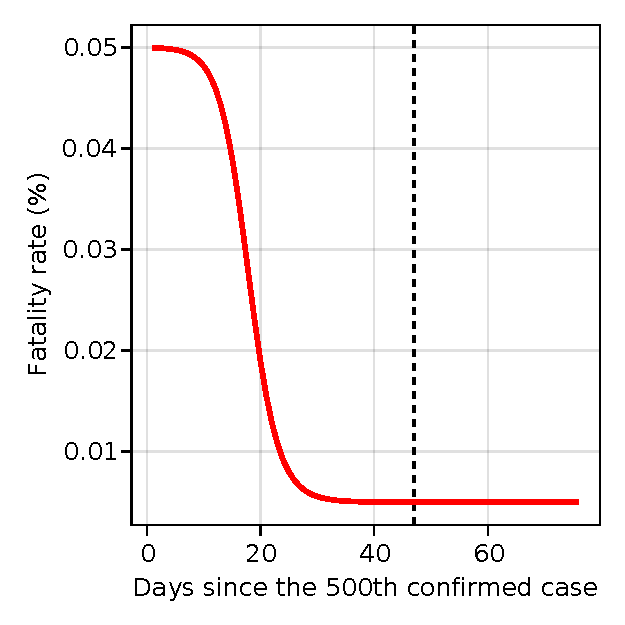
\includegraphics[width=\linewidth]{fb1/maricopa_az/20211216131821.fbmobility1.maricopa_az.fatality_rate.pdf}
        \end{subfigure}
        \subcaption{2nd. version}
    \end{subfigure}

    \begin{subfigure}[b]{\linewidth}
        \centering
        \begin{subfigure}[b]{0.4\linewidth}
            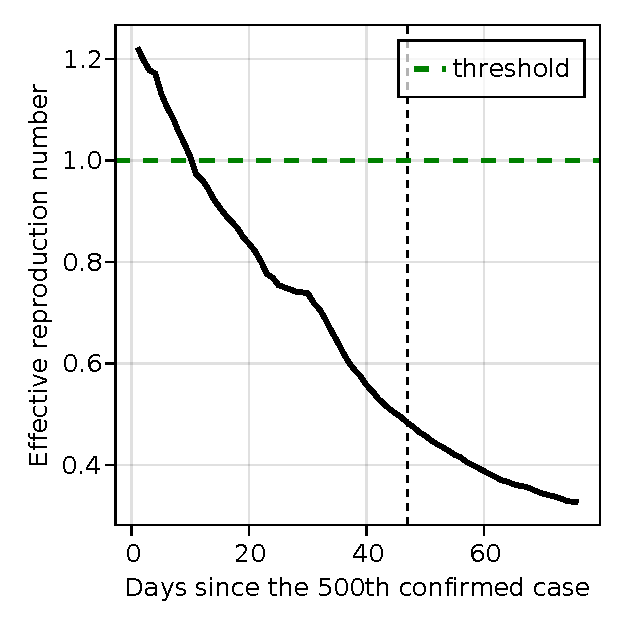
\includegraphics[width=\linewidth]{fb2/maricopa_az/20211216193717.fbmobility2.maricopa_az.R_effective.pdf}
        \end{subfigure}
        \begin{subfigure}[b]{0.4\linewidth}
            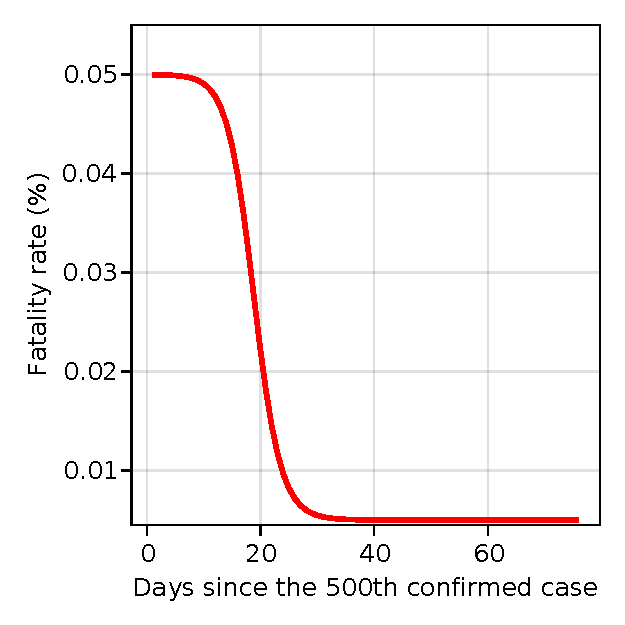
\includegraphics[width=\linewidth]{fb2/maricopa_az/20211216193717.fbmobility2.maricopa_az.fatality_rate.pdf}
        \end{subfigure}
        \subcaption{3rd. version}
    \end{subfigure}

    \caption{The effective reproduction number and the fatality rate for Maricopa (Arizona) learned by different versions of the model}
    \label{fig:R0-and-fatality-maricopa}
\end{figure}
